\documentclass[10pt, letterpaper]{proc}
\usepackage{graphicx}
\usepackage{subcaption}
\usepackage{epstopdf}
\usepackage{comment}
\usepackage[font=small,labelfont=bf]{caption} 
\usepackage{amsmath}
\usepackage{listings}
\usepackage{courier}
\pagestyle{myheadings}
\captionsetup[table]{skip=4pt}
%opening
\title{Stat 462/862 - Assignment 4 Solution}
\author{Chunyang Zhu\\
	 10044873, c.zhu@queensu.ca}

\begin{document}

\maketitle

\section{MH algorithm}
\paragraph{(a)} The target distribution $Bino(n,p)$ was set at $n = 20$ and $p = 0.7$. A description of MH algorithm using independent chains is shown below:

(1) Sample $\theta^\ast \sim q(\theta^\ast | \theta^{(t)})$, where the proposal distribution was a \textbf{uniform distribution} ($min = 0, max = n$).

(2) With probability $ \alpha(\theta^\ast | \theta^{(t)})$, set $ \theta^{(t+1)} = \theta^\ast$, else set $ \theta^{(t+1)} = \theta^{(t)}$. A sequence of simulated values was then generated. It converged to a random variable that had the target distribution. 

The code below was then constructed following this algorithm. 
\begin{lstlisting}[language=R, breaklines=T, basicstyle=\footnotesize\ttfamily]
bino = function (nsim, n, p) 
{
vec = vector("numeric", nsim)
vec[1] = 1
for (i in 2:nsim) {
y <- round (runif(1, min = 0, max = n), digits = 0)
aprob <- min(1, (dbinom(y, n, p)/dbinom(vec[i-1], n, p))/(dunif(y, min = 0, max = n)/dunif(vec[i-1], min = 0, max = n)))
u <- runif(1)
if (u < aprob) 
vec[i] = y
else 
vec[i] = vec[i-1]
}
return(vec)
}
\end{lstlisting}

Table 1 shows the means and variances of estimated (via $mean()$ and $var()$) and theoretical distributions. For a binomial distribution $Bino(n,p)$, the theoretical mean value is $np$ and variance is $np(1-p)$. The values are very close, suggesting that MH algorithm is an effective and reliable algorithm to obtain a sequence of random samples from a probability distribution for which direct sampling is difficult. A detailed comparison in histogram is shown in Figure 1. 

\begin{table}[h]
\centering
\caption{Comparison}
\begin{tabular}{lll}
	\hline  & Mean & Variance \\ 
	\hline Estimated & 14 & 4.2 \\ 
	Theoretical & 14.0422 & 4.256845 \\ 
	\hline 
\end{tabular} 
\end{table}

\begin{figure}[h]
	\centering 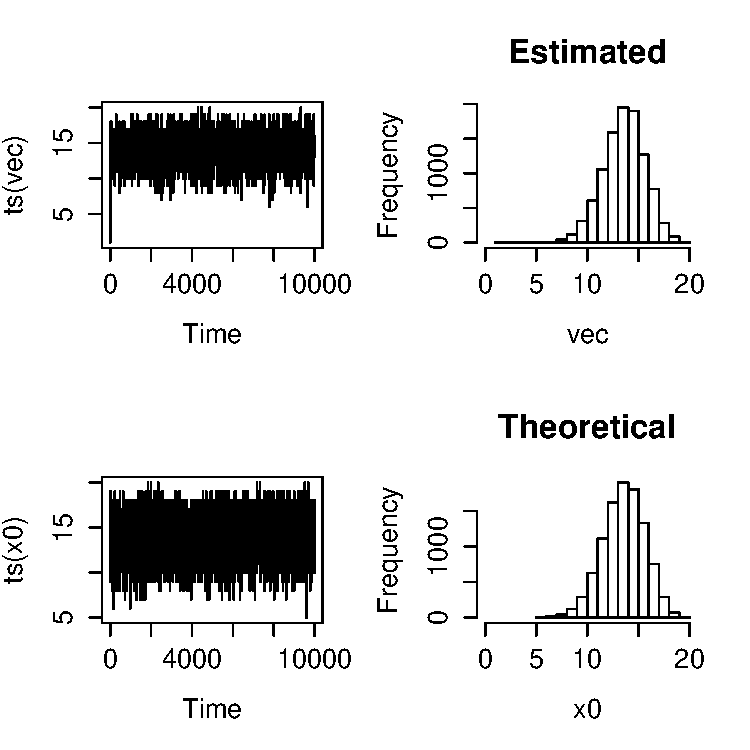
\includegraphics[width = 8cm]{1a}
	\caption{Estimated vs theoretical binomial distribution.}
\end{figure}

\paragraph{(b)}The proposed MH algorithm is shown below:

(1) Sample $\theta^\ast \sim q(\theta^\ast | \theta^{(t)})$, where the proposal distribution was a \textbf{normal distribution} with the mean being the current value in the chain and the variance being 0.25,0.01,100, respectively.

(2) With probability $ \alpha(\theta^\ast | \theta^{(t)})$, set $ \theta^{(t+1)} = \theta^\ast$, else set $ \theta^{(t+1)} = \theta^{(t)}$. A sequence of simulated values was then generated. It converged to a random variable that had the target distribution (standard normal distribution). 

The code below was then constructed following this algorithm. 

\begin{lstlisting}[language=R, breaklines=T, basicstyle=\footnotesize\ttfamily]
stnormal = function (n, sigma)
{
vec = vector("numeric", n)
vec[1] = 0
for (i in 2:n) {
y = rnorm(1, vec[i], sigma )
y = y + vec[i-1]
aprob = min(1, dnorm(y) / dnorm(vec[i-1]))
u = runif(1)
if (u < aprob) 
vec[i] = y
else 
vec[i] = vec[i-1]
}
return(vec)
}
\end{lstlisting}

Table 2 shows the means and variances of estimated and theoretical distributions. The values of these distributions are very close, suggesting that MH algorithm is quite effective and reliable in this case. The mean value is closer to the truth when choosing a larger variance for proposal distribution. A detailed comparison in histogram is shown in Figure 2. 


\begin{table}[h]
	\centering
	\caption{Comparison}
	\begin{tabular}{lrr}
		\hline  & Mean & Variance \\ 
		\hline Theoretical & 0 & 1\\ 
		 Estimated, var = 0.01 & -0.151818512& 1.0431228 \\ 
		 Estimated, var = 0.25 & 0.029003292& 0.9986157 \\ 
		 Estimated, var = 100 & -0.011672239& 0.9705597 \\ 
		\hline 
	\end{tabular} 
\end{table}
             
\begin{figure}
	\centering 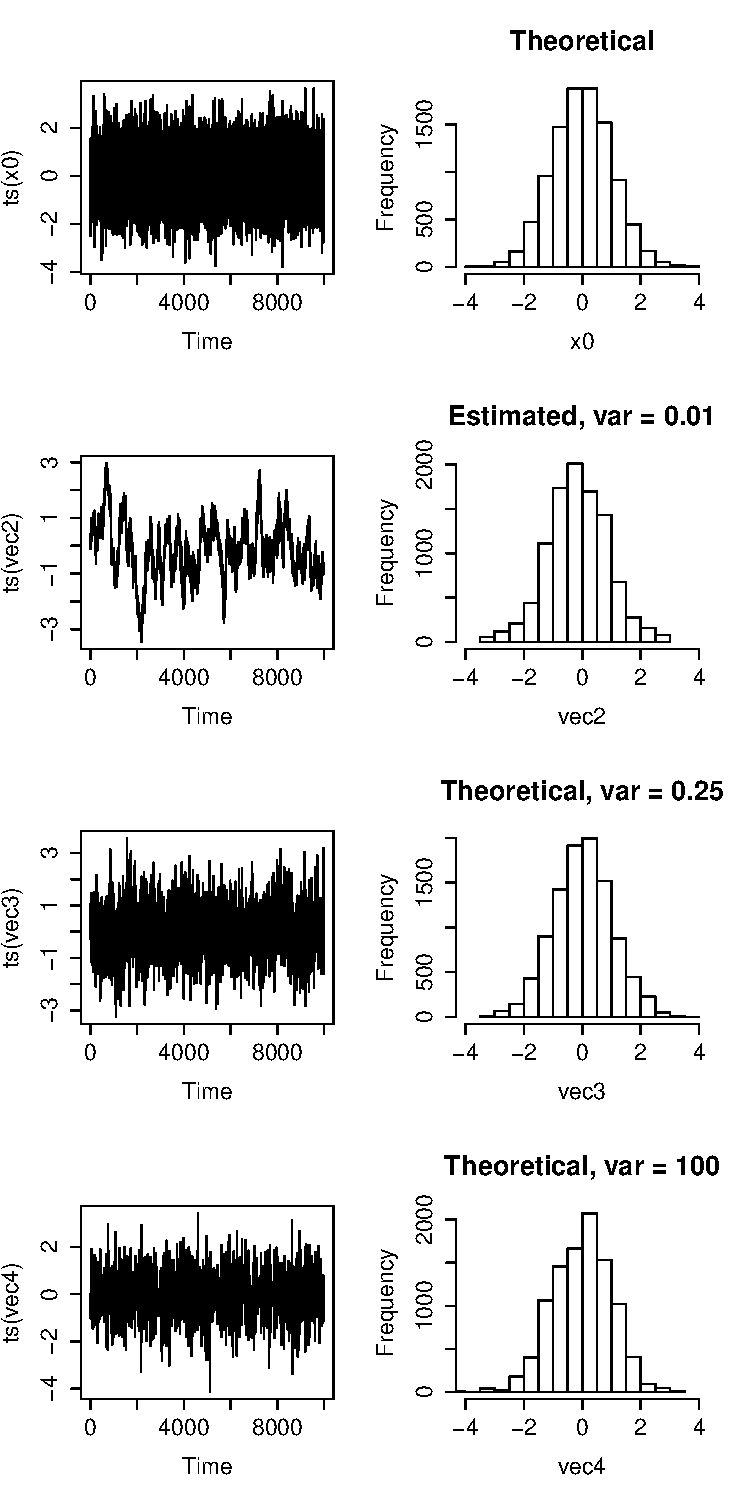
\includegraphics[width = 8.5cm]{1b}
	\caption{Theoretical vs estimated standard normal distribution with different variances.}
\end{figure}

\section{Gibbs sampler}
From the course note we've known that $f(x|\theta)$ follows a Poisson likelihood, while $p(\theta|x)$ follows a gamma distribution(See Eq.(1) and (2)). 
\begin{equation}
f(x|\theta)= (e^{-\theta}\theta^x)/x! 
\end{equation}

\begin{equation}
p(\theta|x) \propto \theta^{x+\alpha-1}e^{-\theta(1+1/\beta)} 
\end{equation}
Notice that in Eq.(1) $\theta$ is considered as a constant and in Eq.(2) $x$ is considered as an constant. Therefore a gibbs sampler can be set up by using the code below. 

In this sampler we set $\alpha = 5$ and $\beta = 1$ for better comparison. Figure 3 shows the histogram of samples of $\theta$ with the true marginal distribution of $\theta$. It turns out the samples of $\theta$ are very close to the true distribution of $\theta$, suggesting that the Gibbs sampler performs very well to obtain a sequence of observations which are approximated from the joint probability distribution of two random variables, when direct sampling is difficult.
\begin{lstlisting}[language=R, breaklines=T, basicstyle=\footnotesize\ttfamily]
N=10000; a=5; b=1
X= vector("numeric",N)  
theta = vector("numeric",N)
theta[1]=rgamma(1,a,b)  
X[1]=rpois(1,theta[1])
for (i in 2:N)
	{
	X[i]=rpois(1,theta[i-1])
	theta[i]=rgamma(1,a+X[i],1+1/b)
	}
theta0 = seq(0,20,by=0.01)
hist(theta[1000:N],breaks = 100, freq = FALSE,xlab=expression(theta), main = "")
lines(theta0,dgamma(theta0,a,b))
\end{lstlisting}

\begin{figure}
	\centering 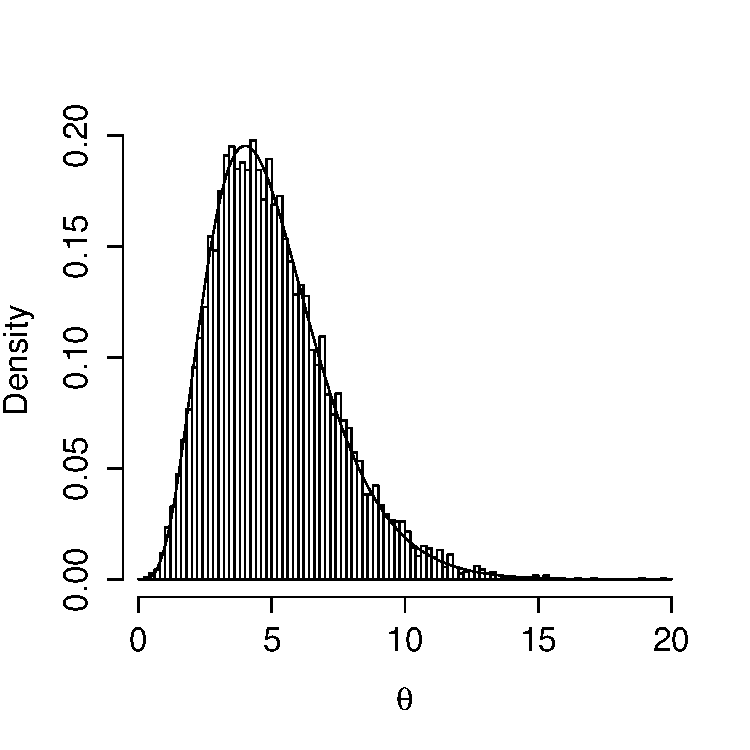
\includegraphics[width = 8cm]{q2}
	\caption{Histogram of samples of $\theta$ and the true marginal distribution of $\theta$.}
\end{figure}

\end{document}
